%%%%%%%%%%%%%%%%%%%%%%%%%%%%%%%%%%%%%
%応用数学 運動座標における運動方程式のメモ
%@maruuusa83
%
%2014.2.5
%%%%%%%%%%%%%%%%%%%%%%%%%%%%%%%%%%%%%

\documentclass[twocolumn,a4j,10pt]{jarticle}
%\documentclass[a4j,10pt]{jarticle}

\usepackage{amsmath,amssymb}
\newtheorem{thm}{定理}

\makeatletter

%パッケージ
\usepackage{bm}
\usepackage[dvipdfmx]{graphicx}
\usepackage{float}

%ヘッダ定義
\usepackage{fancyhdr}
\pagestyle{fancy}
\rhead{applied mathematics}
\cfoot{\thepage}


%文字サイズ定義
\def\section{\@startsection {section}{1}{\z@}{3.5ex plus 1ex minus 2ex}{2.3 ex plus .2ex}{\fontsize{10pt}{0pt}\bf}}
\def\subsection{\@startsection {subsection}{1}{\z@}{3.5ex plus 1ex minus 
2ex}{2.3ex plus .2ex}{\fontsize{10pt}{0pt}\bf}}

%式番号に節番号を含める
\renewcommand{\theequation}{%
\thesection.\arabic{equation}}
\@addtoreset{equation}{section}

%表紙
%
\renewcommand{\maketitle}{\begin{titlepage}%
    \let\footnotesize\small
    \let\footnoterule\relax
    \parindent \z@
    \reset@font
    \null\vfil
    \hrule height 4pt
    \vskip 10\p@
      \LARGE 
      \strut \@title \par
    \begin{flushright}
      \vskip 30\p@
      \strut \@author
    \end{flushright}
    \vskip 5\p@
    \hrule height 4pt
    \vfil
    \begin{flushright}
        {\small \@date}%
    \end{flushright}
  \end{titlepage}%
  \setcounter{footnote}{0}%
}
\makeatother


%ドキュメントの開始%%%%%%%%%%%%%%%%%%%
\begin{document}

%表紙%%%%%%%%%%%%%%%%%%%
\author{marusa}
\title{運動座標系における運動方程式のメモ}
\date{Feb, 2014}

\maketitle

%本文%%%%%%%%%%%%%%%%%%%
\section{前提}
地球から宇宙上にある物体を観測したいとする。

先ず、我々は地球の表面上に座標系を設定して、観測対象の位置
\begin{equation}
  \bm{r}(t) = \sum_{n=1}^{3}x_n \bm{e}_n
  \label{relative_coordinate}
\end{equation}
を観測したという。これは、観測者の状態に依存して様々な値をとるから、\textbf{相対的な観測量}である 

これに対して、絶対静止系に静止している神の観測は
\begin{equation}
  \bm{R}(t) = \sum_{m=1}^{3}X_m \bm{i}_m
  \label{absolute_coordinate}
\end{equation}
である。

地球の中心点の位置を、絶対座標からの位置ベクトルで$\bm{a}$と表し、地球の中心点からの観測者の相対位置ベクトルを$\bm{b}$と表す。

\begin{figure}[H]
  \centering
 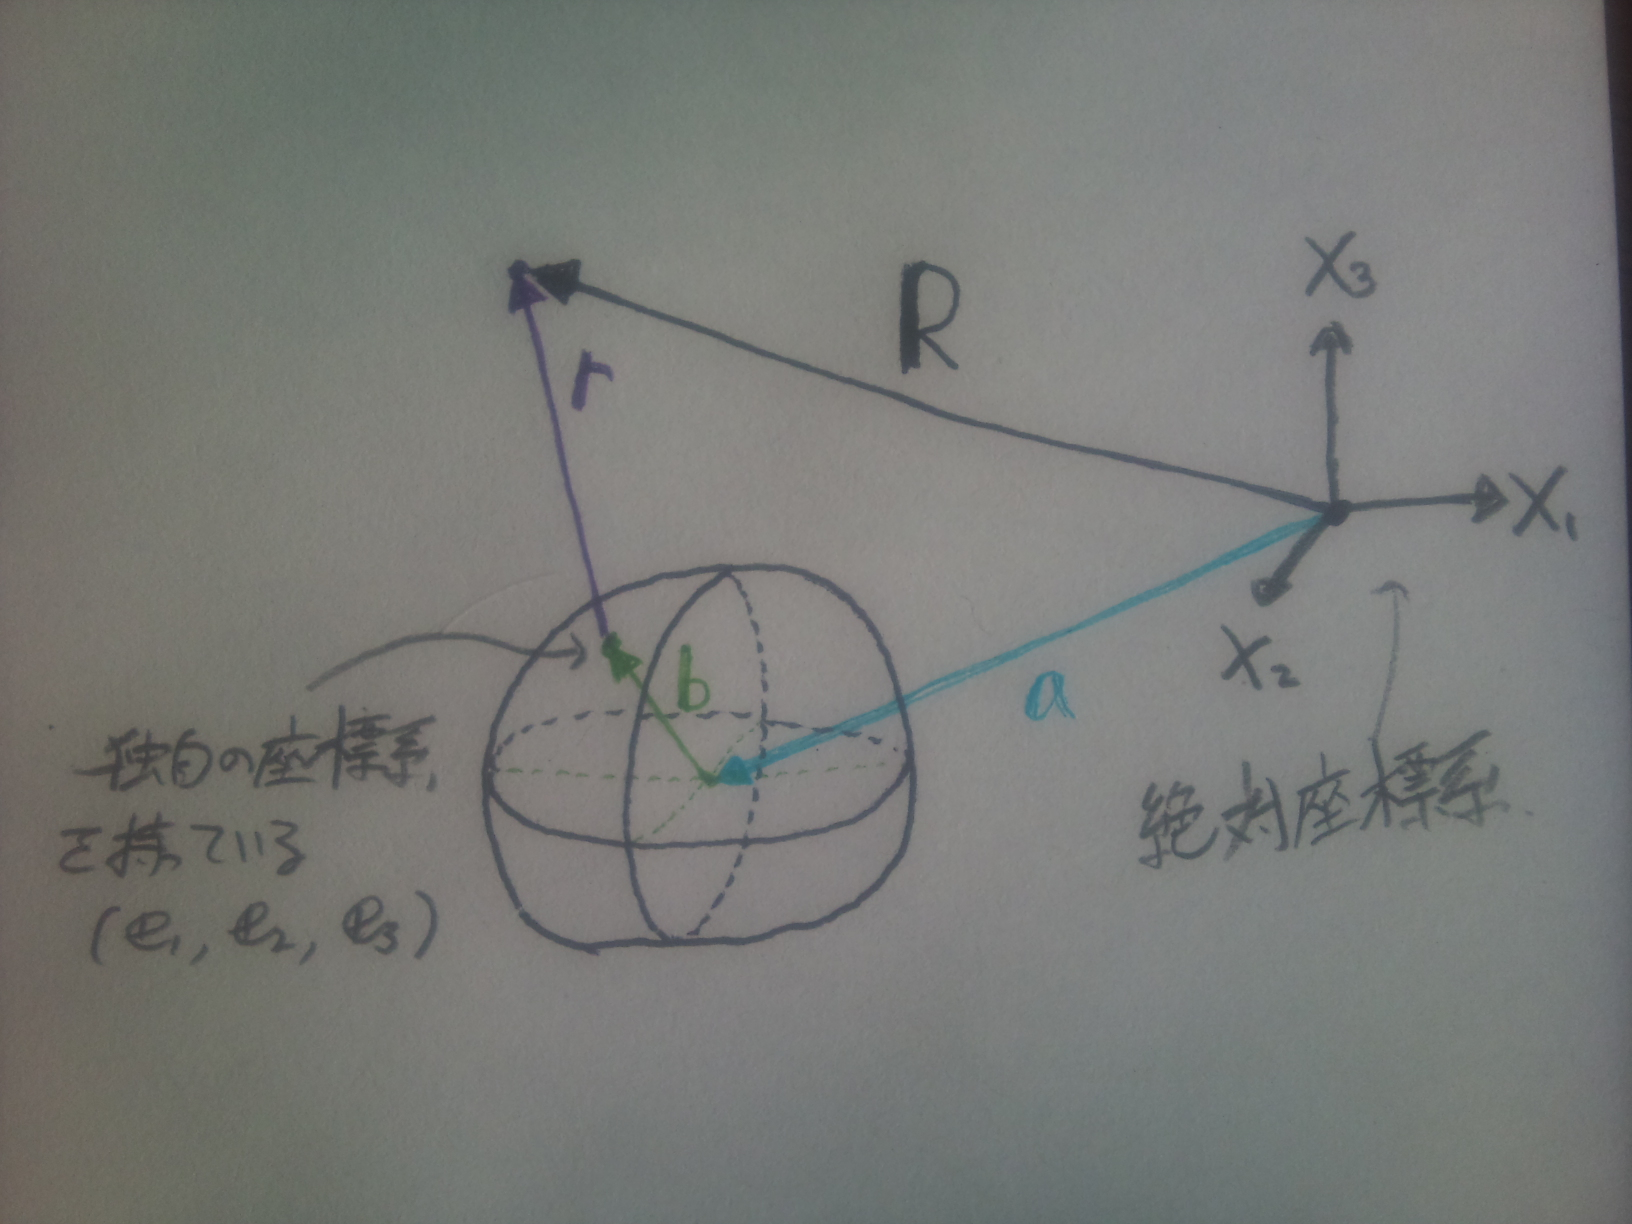
\includegraphics[width=5cm]{./pic/system.jpg}
 \caption{空間の関係図}
 \newline
\end{figure}


\section{目標}
宇宙上に存在している物体の絶対座標系での加速度を求めることが目標である。

ニュートンは、$\bm{F}$=m$\bm{a}$は絶対静止系(またはそれに同等な慣性座標系)において成り立つとした。すなわち、この場合においての\textbf{観測者は運動座標系を持っている}ので正しい運動方程式が得られない。そのため、相対座標$\bm{r}$を用いて観測対象の正しい運動方程式を定める。\newline


\section{幾何学的考察}
地球の位置が絶対座標系において不変だとすると、$\bm{R}$と$\bm{r}$の関係は次のように書くことができる。
\begin{equation}
  \bm{R}(t) = \bm{a} + \bm{b}(t) + \bm{r}(t)
  \label{relation_between_R_r}
\end{equation}
ニュートンの運動方程式における速度は、$\bm{R}$を微分することで得ることができる。我々は$\bm{R}$は知らないものの、$\bm{r}$を知っている。
\begin{eqnarray}
  \frac{\mathrm{d}}{\mathrm{d} t} \bm{R} &=& \frac{\mathrm{d}}{\mathrm{d} t} \left\{ \bm{a} + \bm{b}(t) + \bm{r}(t) \right\} \nonumber \\
 &=& \frac{\mathrm{d}}{\mathrm{d} t} \left\{ \bm{a} + \bm{b}(t) + \sum_{n=1}^{3}x_n (t) \bm{e}_n \right\} \nonumber \\
  &=& \bf{v} \nonumber
\end{eqnarray}
ここで、簡単のために観測者が極点にいた場合を考える。すると$\bm{b}$は一定となるので、
\begin{equation}
  \frac{\mathrm{d}}{\mathrm{d} t} \bm{R} = \bf{v} = \sum_{n=1}^{3}x_n (t) \frac{\mathrm{d}}{\mathrm{d} t} \bm{e}_n
  \label{deff_of_R}
\end{equation}
を得ることができる。\newline


\section{観測者の運動について考える}
ところで、\textbf{円周上を運動する点の位置ベクトルを$\bm{r}$と書くとき、$\bm{r}$の速度ベクトル$\frac{\mathrm{d}\bm{r}}{\mathrm{d}t}$は$\bm{r}$に垂直}であるから、
\begin{equation}
  \frac{\mathrm{d} \bm{e}_1}{\mathrm{d} t} = (係数)\bm{e}_2 + (係数)\bm{e}_3 \nonumber
\end{equation}

と表すことができる。この係数を、基底aに対する基底bの貢献度:$\Omega_{ab}$と書くことにして他の軸についてもまとめると、

\begin{equation}
  \left\{ \begin{array}{rl}
\frac{\mathrm{d} }{\mathrm{d} t} \bm{e}_1 = \Omega_{12} \bm{e}_2 + \Omega_{13} \bm{e}_3 \\
\frac{\mathrm{d} }{\mathrm{d} t} \bm{e}_2 = \Omega_{23} \bm{e}_3 + \Omega_{21} \bm{e}_1 \\
\frac{\mathrm{d} }{\mathrm{d} t} \bm{e}_3 = \Omega_{31} \bm{e}_1 + \Omega_{32} \bm{e}_2
  \label{speed_of_observer}
  \end{array} \right.
\end{equation}\newline
を得ることができる。\newline

もう少しこの式を整理しよう。基底ベクトルは直行するので、その内積の値は0である。これを時間$t$で微分すると、
\begin{equation}
  \frac{\mathrm{d} \bm{e}_1}{\mathrm{d} t} \bm{e}_2 + \bm{e}_1 \frac{\mathrm{d} \bm{e}_2}{\mathrm{d} t} = 0 \nonumber
\end{equation}
を得る。

ところで、それぞれの式において次のように左辺の項が1つ消えるように基底ベクトルの内積をとると、次のような結果が得られる。
\begin{eqnarray}
  \frac{\mathrm{d} \bm{e}_1}{\mathrm{d} t} \cdot \bm{e}_2 &=& \Omega_{12} \bm{e}_2 \cdot \bm{e}_2 + \Omega_{13} \bm{e}_3 \cdot \bm{e}_2 \nonumber \\
  &=& \Omega_{12} \nonumber
\end{eqnarray}

この2つの性質を用いると、次の性質を持つことがわかる。
\begin{eqnarray}
  \Omega_{12} + \Omega_{21} = 0 \nonumber \\
  \Omega_{23} + \Omega_{32} = 0 \nonumber \\
  \Omega_{31} + \Omega_{13} = 0 \nonumber
\end{eqnarray}
このことから、式(\ref{speed_of_observer})は次のように書き直すことができる。

\begin{equation}
  \left\{ \begin{array}{rl}
\frac{\mathrm{d} }{\mathrm{d} t} \bm{e}_1 = \Omega_{12} \bm{e}_2 - \Omega_{31} \bm{e}_3 \\
\frac{\mathrm{d} }{\mathrm{d} t} \bm{e}_2 = \Omega_{23} \bm{e}_3 - \Omega_{12} \bm{e}_1 \\
\frac{\mathrm{d} }{\mathrm{d} t} \bm{e}_3 = \Omega_{31} \bm{e}_1 - \Omega_{23} \bm{e}_2
  \label{speed_of_observer}
  \end{array} \right.
\end{equation}\newline




\end{document}


























